\documentclass[12pt]{article}\usepackage[]{graphicx}\usepackage[]{color}
%% maxwidth is the original width if it is less than linewidth
%% otherwise use linewidth (to make sure the graphics do not exceed the margin)
\makeatletter
\def\maxwidth{ %
  \ifdim\Gin@nat@width>\linewidth
    \linewidth
  \else
    \Gin@nat@width
  \fi
}
\makeatother

\definecolor{fgcolor}{rgb}{0.345, 0.345, 0.345}
\newcommand{\hlnum}[1]{\textcolor[rgb]{0.686,0.059,0.569}{#1}}%
\newcommand{\hlstr}[1]{\textcolor[rgb]{0.192,0.494,0.8}{#1}}%
\newcommand{\hlcom}[1]{\textcolor[rgb]{0.678,0.584,0.686}{\textit{#1}}}%
\newcommand{\hlopt}[1]{\textcolor[rgb]{0,0,0}{#1}}%
\newcommand{\hlstd}[1]{\textcolor[rgb]{0.345,0.345,0.345}{#1}}%
\newcommand{\hlkwa}[1]{\textcolor[rgb]{0.161,0.373,0.58}{\textbf{#1}}}%
\newcommand{\hlkwb}[1]{\textcolor[rgb]{0.69,0.353,0.396}{#1}}%
\newcommand{\hlkwc}[1]{\textcolor[rgb]{0.333,0.667,0.333}{#1}}%
\newcommand{\hlkwd}[1]{\textcolor[rgb]{0.737,0.353,0.396}{\textbf{#1}}}%

\usepackage{framed}
\makeatletter
\newenvironment{kframe}{%
 \def\at@end@of@kframe{}%
 \ifinner\ifhmode%
  \def\at@end@of@kframe{\end{minipage}}%
  \begin{minipage}{\columnwidth}%
 \fi\fi%
 \def\FrameCommand##1{\hskip\@totalleftmargin \hskip-\fboxsep
 \colorbox{shadecolor}{##1}\hskip-\fboxsep
     % There is no \\@totalrightmargin, so:
     \hskip-\linewidth \hskip-\@totalleftmargin \hskip\columnwidth}%
 \MakeFramed {\advance\hsize-\width
   \@totalleftmargin\z@ \linewidth\hsize
   \@setminipage}}%
 {\par\unskip\endMakeFramed%
 \at@end@of@kframe}
\makeatother

\definecolor{shadecolor}{rgb}{.97, .97, .97}
\definecolor{messagecolor}{rgb}{0, 0, 0}
\definecolor{warningcolor}{rgb}{1, 0, 1}
\definecolor{errorcolor}{rgb}{1, 0, 0}
\newenvironment{knitrout}{}{} % an empty environment to be redefined in TeX

\usepackage{alltt}

\usepackage{amssymb,amsmath}
\usepackage{enumerate}
\usepackage{float}
\usepackage{verbatim}
\usepackage{setspace}

%% LaTeX margin settings:
  \setlength{\textwidth}{7.0in}
\setlength{\textheight}{9in}
\setlength{\oddsidemargin}{-.5in}
\setlength{\evensidemargin}{0in}
\setlength{\topmargin}{-1.5cm}

%% tell knitr to use smaller font for code chunks
\def\fs{\footnotesize}
\def\R{{\sf R}}
\newcommand{\bfbeta}{\mbox{\boldmath $\beta$}}
\newcommand{\bfD}{\mbox{\boldmath $D$}}
\newcommand{\bfL}{\mbox{\boldmath $L$}}
\newcommand{\bfR}{\mbox{\boldmath $R$}}
\newcommand{\bfmu}{\mbox{\boldmath $\mu$}}
\newcommand{\bfv}{\mbox{\boldmath $V$}}
\newcommand{\bfX}{\mbox{\boldmath $X$}}
\newcommand{\bfy}{\mbox{\boldmath $y$}}
\newcommand{\bfb}{\mbox{\boldmath $b$}}
\IfFileExists{upquote.sty}{\usepackage{upquote}}{}
\begin{document}


  
  
\begin{center}
\large{Bayes: Homework $1$} \\
Leslie Gains-Germain
\end{center}

\begin{doublespacing}

\begin{enumerate}

\item The \verb+dhyper(x, m, n, k, log = FALSE)+ function gives the probability of drawing $X=x$ white balls without replacement from $k$ draws out of an urn with $m$ white balls and $n$ black balls.

\item My function is below. The default value for $x$ is $1$.

\begin{knitrout}\footnotesize
\definecolor{shadecolor}{rgb}{0.969, 0.969, 0.969}\color{fgcolor}\begin{kframe}
\begin{alltt}
\hlstd{hyper.fun} \hlkwb{<-} \hlkwa{function}\hlstd{(}\hlkwc{theta}\hlstd{,} \hlkwc{x}\hlstd{=}\hlnum{1}\hlstd{) \{}
  \hlkwd{choose}\hlstd{(theta, x)} \hlopt{*} \hlkwd{choose}\hlstd{((}\hlnum{12}\hlopt{-}\hlstd{theta), (}\hlnum{5}\hlopt{-}\hlstd{x))} \hlopt{/} \hlkwd{choose}\hlstd{(}\hlnum{12}\hlstd{,} \hlnum{5}\hlstd{)}
\hlstd{\}}
\hlkwd{hyper.fun}\hlstd{(}\hlnum{0.1}\hlstd{)}
\end{alltt}
\begin{verbatim}
## [1] 0.0601
\end{verbatim}
\end{kframe}
\end{knitrout}

\item 

\begin{knitrout}\footnotesize
\definecolor{shadecolor}{rgb}{0.969, 0.969, 0.969}\color{fgcolor}\begin{kframe}
\begin{alltt}
\hlstd{theta.vec} \hlkwb{<-} \hlkwd{matrix}\hlstd{(}\hlnum{0}\hlopt{:}\hlnum{12}\hlstd{)}
\hlstd{nice.table} \hlkwb{<-} \hlkwd{matrix}\hlstd{(}\hlnum{NA}\hlstd{,} \hlkwc{nrow}\hlstd{=}\hlnum{13}\hlstd{,} \hlkwc{ncol}\hlstd{=}\hlnum{6}\hlstd{)}
\hlkwa{for}\hlstd{(i} \hlkwa{in} \hlnum{1}\hlopt{:}\hlnum{6}\hlstd{)\{}
  \hlstd{nice.table[,i]} \hlkwb{<-} \hlkwd{apply}\hlstd{(theta.vec,} \hlnum{1}\hlstd{, hyper.fun,} \hlkwc{x}\hlstd{=i}\hlopt{-}\hlnum{1}\hlstd{)}
\hlstd{\}}
\end{alltt}
\end{kframe}
\end{knitrout}

\item 

\begin{knitrout}\footnotesize
\definecolor{shadecolor}{rgb}{0.969, 0.969, 0.969}\color{fgcolor}\begin{kframe}
\begin{alltt}
\hlstd{col.sums} \hlkwb{<-} \hlkwd{apply}\hlstd{(nice.table,} \hlnum{2}\hlstd{, sum)}
\hlstd{col.sums}
\end{alltt}
\begin{verbatim}
## [1] 2.17 2.17 2.17 2.17 2.17 2.17
\end{verbatim}
\begin{alltt}
\hlstd{row.sums} \hlkwb{<-} \hlkwd{apply}\hlstd{(nice.table,} \hlnum{1}\hlstd{, sum)}
\hlstd{row.sums}
\end{alltt}
\begin{verbatim}
##  [1] 1 1 1 1 1 1 1 1 1 1 1 1 1
\end{verbatim}
\end{kframe}
\end{knitrout}

The rows sum to one because for a given a value of theta, each row describes the probability of drawing $x$ gold marbles. When we sum over the entire support, $0$ to $5$, we get $1$ because the probability that some event in the sample space occurs is $1$. When we sum across the columns, we are summing over the likelihood of different values of theta given $x$ is fixed. These do not sum to $1$ because the likelihood function is not a probability mass function.

\item Given a fixed $x$, $\theta$ is the independent variable, and the likelihood function, $L(\theta|x)$ is simply a function of $\theta$. It is not a probability mass function because it does not describe the probabilities for a set of possible outcomes of a random event. Instead, it is a function that describes the likelihood for possible values of $\theta$ given the random event has occurred and $x$ has been observed. We usually use the notation $f(x|\theta)$ for a probability mass function and $L(\theta|x)$ for a likelihood function.

\item We often use the maximum likelihood principle to estimate $\theta$. We look at the values of the likelihood function across the possible values of $\theta$, and we choose the $\theta$ that maximizes the likelihood function (given $X=x$ has been observed). The value of $\theta$ that maximizes the likelihood function is our best guess for the true value of $\theta$. 

\item An estimator is a random variable defined prior to data collection. For example, $\bar{X}$ is a common estimator, it is a function of the data before the data have been observed. An estimate is a realization of the estimator and is calculated after the data are observed. For example, $\bar{x}$ is a point estimate for a population mean, and it is calculated with observed data $x_1, x_2,.., x_n$.

\item The maximum likelihood estimator could be $0, 2, 5, 7, 10$, or $12$. I found these by looking at the above table, and they correspond to the $6$ possible values of X as in the following table. For example, if we draw $X=1$, then the likelihood function is maximized at $\hat{\theta}=2$.

\begin{table} [H]
\centering
\begin{tabular}{c c}
X & $\hat{\theta}$ \\
\hline
0 & 0 \\
1 & 2 \\
2 & 5 \\
3 & 7 \\
4 & 10 \\
5 & 12 \\
\hline
\end{tabular}
\end{table}

\item Since we are drawing $5$ marbles out of the bucket (with a total of $12$ marbles), there are $792$ possible samples that could be drawn. I'm going to suppose the true value of $\theta$ is $7$, and simulate $500$ samples. For each sample, I will find the maximum likelihood estimate and build a histogram to give you an idea of what the sampling distribution of ML estimates would look like. \\

Here's an approximate sampling distribution of maximum likelihood {\it estimates} constructed with $500$ simulations. It is centered at the true number of gold balls, $7$, and the MLE's farther from $7$ are less likely to occur.

\begin{knitrout}\footnotesize
\definecolor{shadecolor}{rgb}{0.969, 0.969, 0.969}\color{fgcolor}\begin{kframe}
\begin{alltt}
\hlkwd{set.seed}\hlstd{(}\hlnum{5}\hlstd{)}
\hlstd{sims} \hlkwb{<-} \hlkwd{rhyper}\hlstd{(}\hlnum{500}\hlstd{,} \hlnum{7}\hlstd{,} \hlnum{5}\hlstd{,} \hlnum{5}\hlstd{)}
\hlstd{mles} \hlkwb{<-} \hlkwd{ifelse}\hlstd{(sims}\hlopt{==}\hlnum{0}\hlstd{,} \hlnum{0}\hlstd{,}
               \hlkwd{ifelse}\hlstd{(sims}\hlopt{==}\hlnum{1}\hlstd{,} \hlnum{2}\hlstd{,}
                      \hlkwd{ifelse}\hlstd{(sims}\hlopt{==}\hlnum{2}\hlstd{,} \hlnum{5}\hlstd{,}
                             \hlkwd{ifelse}\hlstd{(sims}\hlopt{==}\hlnum{3}\hlstd{,} \hlnum{7}\hlstd{,}
                                    \hlkwd{ifelse}\hlstd{(sims}\hlopt{==}\hlnum{4}\hlstd{,} \hlnum{10}\hlstd{,}
                                           \hlkwd{ifelse}\hlstd{(sims}\hlopt{==}\hlnum{5}\hlstd{,} \hlnum{12}\hlstd{,} \hlnum{0}\hlstd{))))))}
\hlkwd{require}\hlstd{(mosaic)}
\hlkwd{dotPlot}\hlstd{(mles,} \hlkwc{main}\hlstd{=}\hlstr{"Approx Sampling Distribution of MLES if theta=7"}\hlstd{,} \hlkwc{cex}\hlstd{=}\hlnum{2}\hlstd{,} \hlkwc{pch}\hlstd{=}\hlnum{5}\hlstd{)}
\end{alltt}
\end{kframe}
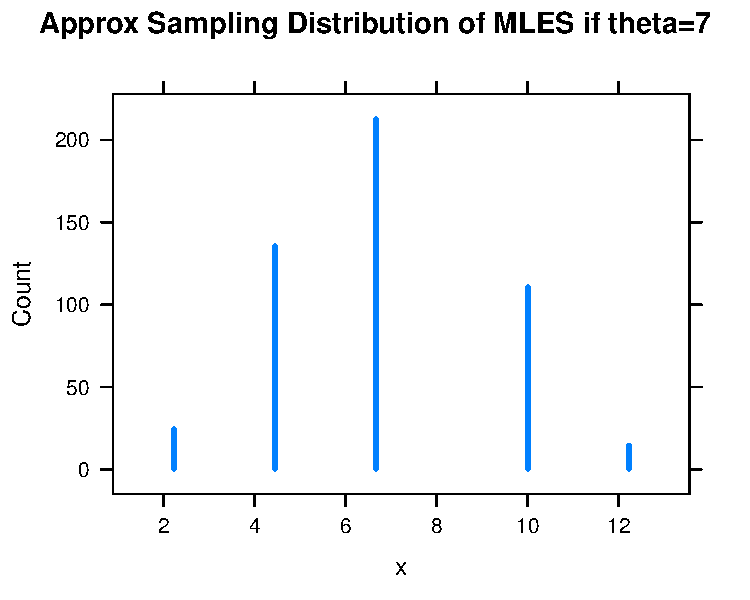
\includegraphics[width=.5\linewidth]{figure/sim-1} 

\end{knitrout}

I think that the best way to display the sampling distribution of the maximum likelihood {\it estimator} is through a table. We would essentially just take the table that we used to describe the likelihood function previously, and list the possible values for the ML estimator at the top. For each true value of $\theta$, the long run relative frequencies of each possible value of the ML estimator are shown in the rows of the table.

% latex table generated in R 3.2.2 by xtable 1.7-4 package
% Tue Sep  1 14:55:04 2015
\begin{table}[ht]
\centering
\begin{tabular}{rrrrrrr}
  \hline
 & 0 & 2 & 5 & 7 & 10 & 12 \\ 
  \hline
0 & 1.00 & 0.00 & 0.00 & 0.00 & 0.00 & 0.00 \\ 
  1 & 0.58 & 0.42 & 0.00 & 0.00 & 0.00 & 0.00 \\ 
  2 & 0.32 & 0.53 & 0.15 & 0.00 & 0.00 & 0.00 \\ 
  3 & 0.16 & 0.48 & 0.32 & 0.05 & 0.00 & 0.00 \\ 
  4 & 0.07 & 0.35 & 0.42 & 0.14 & 0.01 & 0.00 \\ 
  5 & 0.03 & 0.22 & 0.44 & 0.27 & 0.04 & 0.00 \\ 
  6 & 0.01 & 0.11 & 0.38 & 0.38 & 0.11 & 0.01 \\ 
  7 & 0.00 & 0.04 & 0.27 & 0.44 & 0.22 & 0.03 \\ 
  8 & 0.00 & 0.01 & 0.14 & 0.42 & 0.35 & 0.07 \\ 
  9 & 0.00 & 0.00 & 0.05 & 0.32 & 0.48 & 0.16 \\ 
  10 & 0.00 & 0.00 & 0.00 & 0.15 & 0.53 & 0.32 \\ 
  11 & 0.00 & 0.00 & 0.00 & 0.00 & 0.42 & 0.58 \\ 
  12 & 0.00 & 0.00 & 0.00 & 0.00 & 0.00 & 1.00 \\ 
   \hline
\end{tabular}
\end{table}



\item \begin{enumerate} \item The maximum likelihood estimate is $2$. 

\item Given $x$ is $1$, this plot shows the values of the likelihood function over the range of possible values of $\theta$. You can clearly see that the maximum likelihood estimate is $2$. A histogram wouldn't make sense here. I {\it think} it would show you how many likelihoods were in each 'bin', and the largest bin would be the $0$ to $0.1$ bin because there are so many zeros. This is not useful information at all. 

\begin{knitrout}\footnotesize
\definecolor{shadecolor}{rgb}{0.969, 0.969, 0.969}\color{fgcolor}\begin{kframe}
\begin{alltt}
\hlkwd{plot}\hlstd{(}\hlnum{0}\hlopt{:}\hlnum{12}\hlstd{, nice.table[,}\hlnum{2}\hlstd{],} \hlkwc{xlab}\hlstd{=}\hlstr{"theta"}\hlstd{,} \hlkwc{ylab}\hlstd{=}\hlstr{"likelihood given x=1"}\hlstd{)}
\end{alltt}
\end{kframe}
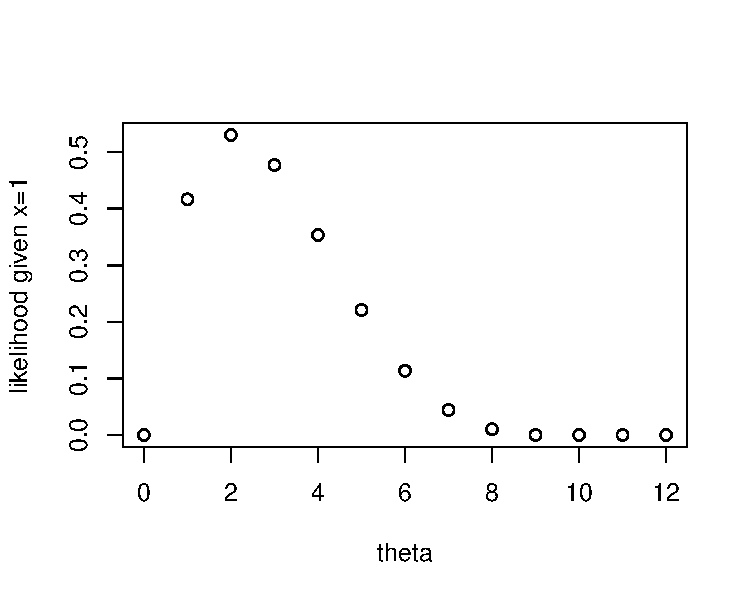
\includegraphics[width=.5\linewidth]{figure/lfun-1} 

\end{knitrout}

\item The normalized likelihood function is just a rescaled version of the likelihood function so that the likelihood sums to $1$ over all possible $\theta$ values.

\begin{knitrout}\footnotesize
\definecolor{shadecolor}{rgb}{0.969, 0.969, 0.969}\color{fgcolor}\begin{kframe}
\begin{alltt}
\hlkwd{plot}\hlstd{(}\hlnum{0}\hlopt{:}\hlnum{12}\hlstd{, nice.table[,}\hlnum{2}\hlstd{]}\hlopt{/}\hlkwd{sum}\hlstd{(nice.table[,}\hlnum{2}\hlstd{]),} \hlkwc{xlab}\hlstd{=}\hlstr{"theta"}\hlstd{,} \hlkwc{ylab}\hlstd{=}\hlstr{"normalized likelihood"}\hlstd{)}
\end{alltt}
\end{kframe}
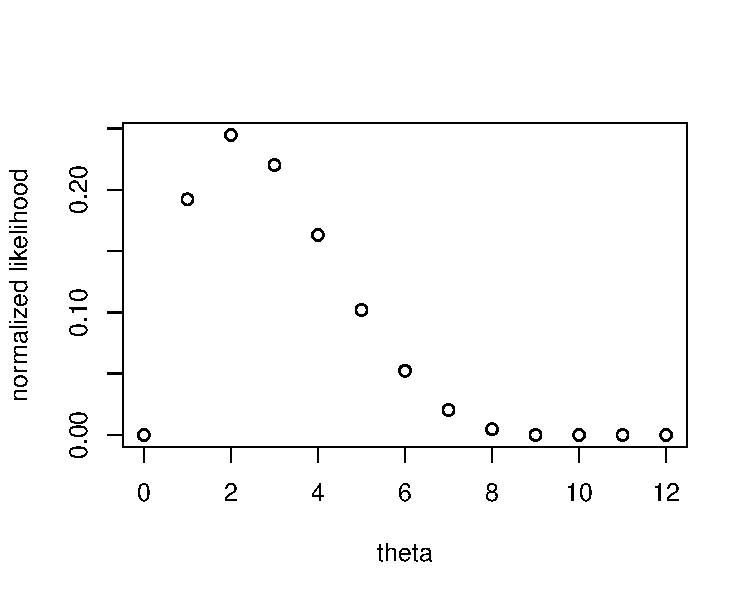
\includegraphics[width=.5\linewidth]{figure/norm-1} 

\end{knitrout}


\end{enumerate}

\item \begin{enumerate}

\item Consider the simple linear regression model: \\

$y_i = \beta_0 + \beta_1x_i + e_i$ \\

I simulated data to investigate this problem.

\begin{knitrout}\footnotesize
\definecolor{shadecolor}{rgb}{0.969, 0.969, 0.969}\color{fgcolor}\begin{kframe}
\begin{alltt}
\hlstd{x} \hlkwb{<-} \hlnum{1}\hlopt{:}\hlnum{20}
\hlstd{y} \hlkwb{<-} \hlnum{3} \hlopt{+} \hlnum{2}\hlopt{*}\hlstd{x} \hlopt{+} \hlkwd{rnorm}\hlstd{(}\hlnum{20}\hlstd{,}\hlnum{0}\hlstd{,}\hlnum{5}\hlstd{)}
\hlstd{data.sim} \hlkwb{<-} \hlkwd{data.frame}\hlstd{(}\hlkwd{cbind}\hlstd{(x,y))}
\hlkwd{plot}\hlstd{(x,y)}
\end{alltt}
\end{kframe}
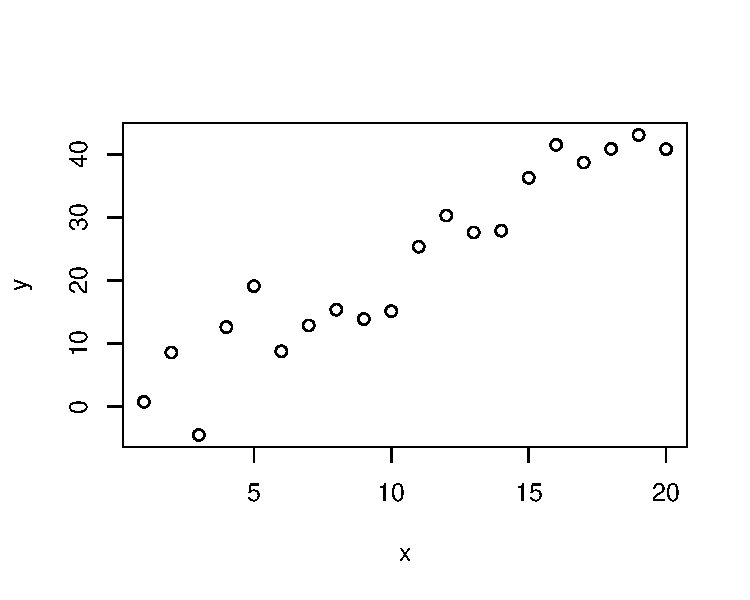
\includegraphics[width=.5\linewidth]{figure/sim2-1} 
\begin{kframe}\begin{alltt}
\hlstd{lm.fit} \hlkwb{<-} \hlkwd{lm}\hlstd{(y} \hlopt{~} \hlstd{x,} \hlkwc{data} \hlstd{= data.sim)}
\hlkwd{coef}\hlstd{(lm.fit)}
\end{alltt}
\begin{verbatim}
## (Intercept)           x 
##       -1.63        2.32
\end{verbatim}
\begin{alltt}
\hlstd{glm.fit} \hlkwb{<-} \hlkwd{glm}\hlstd{(y} \hlopt{~} \hlstd{x,} \hlkwc{data} \hlstd{= data.sim,} \hlkwc{family} \hlstd{=} \hlstr{"gaussian"}\hlstd{)}
\hlkwd{coef}\hlstd{(lm.fit)}
\end{alltt}
\begin{verbatim}
## (Intercept)           x 
##       -1.63        2.32
\end{verbatim}
\end{kframe}
\end{knitrout}


The \verb+lm()+ procedure finds the ordinary least squares estimates for $\beta_0$ and $\beta_1$ by minimizing the sum of squared residuals. The distributional assumption is that $\epsilon_i \sim (0, \sigma^2)$. Note that the assumption for normality is not actually needed to calculate the OLS estimates - the assumption of normality is only made in order to calculate p-values and confidence intervals. \\

In the \verb+glm()+ procedure, we specify \verb+family="gaussian"+ and an identity link function, so the distributional assumption is: $\epsilon_i \sim N(0, \sigma^2)$. The default procedure used to find the estimates in \verb+glm()+ is maximum likelihood estimation, and it does this using iteratively reweighted least squares. Because we are assuming normally distributed errors, the maximum likelihood estimate is the same as the ordinary least squares estimate from \verb+lm+.

\item The \verb+lm+ procedure gives t-based confidence intervals when the \verb+confint+ function is used. It calculates these intervals by adding and subtracting from the estimates the standard error multiplied by the t multiplier. \\

The \verb+glm+ procedure gives likelihood based confidence intervals. It finds these by plotting the likelihood over the entire parameter space, and then it finds the $2.5$th and $97.5$th percentiles from the likelihood function. I think it looks at the marginal likelihood function separately for each parameter to do this?

\begin{knitrout}\footnotesize
\definecolor{shadecolor}{rgb}{0.969, 0.969, 0.969}\color{fgcolor}\begin{kframe}
\begin{alltt}
\hlkwd{confint}\hlstd{(lm.fit)}
\end{alltt}
\begin{verbatim}
##             2.5 % 97.5 %
## (Intercept) -6.32   3.06
## x            1.93   2.71
\end{verbatim}
\begin{alltt}
\hlkwd{confint}\hlstd{(glm.fit)}
\end{alltt}


{\ttfamily\noindent\itshape\color{messagecolor}{\#\# Waiting for profiling to be done...}}\begin{verbatim}
##             2.5 % 97.5 %
## (Intercept) -6.00   2.74
## x            1.96   2.69
\end{verbatim}
\end{kframe}
\end{knitrout}

\end{enumerate}

\item This is how I think of Bayes Theorem:
\begin{align*}
f(\theta|x) &= \frac{f(x|\theta)*f(\theta)}{f(x)}
\end{align*}

A lot of books use p`s for probability mass functions. In the bucket problem, both $X$ and $\theta$ are discrete random variables, so the notation I would use for this problem is as follows.

\begin{align*}
p(\theta|x) &= \frac{p(x|\theta)*p(\theta)}{p(x)}
\end{align*}

\item In the bucket problem, we replace $p(x|\theta)$ with the likelihood function, $L(\theta|x)$, which we know to be a hypergeometric distribution. The marginal distribution in the denominator is found by finding the joint distribution of $x$ and $\theta$ and then summing over all values of $\theta$.

\begin{align*}
p(\theta|x) &= \frac{p(x|\theta)*p(\theta)}{p(x)} \\
            &= \frac{L(\theta|x)*p(\theta)}{\sum_{\theta \in \Theta} L(\theta|x)*p(\theta)} = \frac{\frac{{\theta \choose x} {12-\theta \choose 5-x}} {{12 \choose 5}} * p(\theta)} {\sum_{\theta=0}^{\theta=12} \frac{{\theta \choose x} {1-\theta \choose 5-x}} {{12 \choose 5}} * p(\theta)}
\end{align*}

\item \begin{enumerate}

\item
\begin{knitrout}\footnotesize
\definecolor{shadecolor}{rgb}{0.969, 0.969, 0.969}\color{fgcolor}\begin{kframe}
\begin{alltt}
\hlstd{theta} \hlkwb{<-} \hlnum{0}\hlopt{:}\hlnum{12}
\hlstd{priors} \hlkwb{<-} \hlkwd{c}\hlstd{(}\hlnum{0}\hlstd{,} \hlnum{0}\hlstd{,} \hlnum{1}\hlopt{/}\hlnum{36}\hlstd{,} \hlnum{2}\hlopt{/}\hlnum{36}\hlstd{,} \hlnum{3}\hlopt{/}\hlnum{36}\hlstd{,} \hlnum{4}\hlopt{/}\hlnum{36}\hlstd{,} \hlnum{5}\hlopt{/}\hlnum{36}\hlstd{,} \hlnum{6}\hlopt{/}\hlnum{36}\hlstd{,} \hlnum{5}\hlopt{/}\hlnum{36}\hlstd{,} \hlnum{4}\hlopt{/}\hlnum{36}\hlstd{,} \hlnum{3}\hlopt{/}\hlnum{36}\hlstd{,} \hlnum{2}\hlopt{/}\hlnum{36}\hlstd{,} \hlnum{1}\hlopt{/}\hlnum{36}\hlstd{)}
\hlstd{likelihood} \hlkwb{<-} \hlkwd{apply}\hlstd{(theta.vec,} \hlnum{1}\hlstd{, hyper.fun,} \hlkwc{x} \hlstd{=} \hlnum{1}\hlstd{)}
\hlstd{product} \hlkwb{<-} \hlstd{likelihood}\hlopt{*}\hlstd{priors}
\hlstd{posterior} \hlkwb{<-} \hlstd{likelihood}\hlopt{*}\hlstd{priors}\hlopt{/}\hlkwd{sum}\hlstd{(product)}
\hlstd{dice.sum} \hlkwb{<-} \hlkwd{cbind}\hlstd{(theta, priors, likelihood, product, posterior)}
\hlstd{dice.sum}
\end{alltt}
\begin{verbatim}
##       theta priors likelihood product posterior
##  [1,]     0 0.0000     0.0000 0.00000    0.0000
##  [2,]     1 0.0000     0.4167 0.00000    0.0000
##  [3,]     2 0.0278     0.5303 0.01473    0.1230
##  [4,]     3 0.0556     0.4773 0.02652    0.2213
##  [5,]     4 0.0833     0.3535 0.02946    0.2459
##  [6,]     5 0.1111     0.2210 0.02455    0.2049
##  [7,]     6 0.1389     0.1136 0.01578    0.1317
##  [8,]     7 0.1667     0.0442 0.00737    0.0615
##  [9,]     8 0.1389     0.0101 0.00140    0.0117
## [10,]     9 0.1111     0.0000 0.00000    0.0000
## [11,]    10 0.0833     0.0000 0.00000    0.0000
## [12,]    11 0.0556     0.0000 0.00000    0.0000
## [13,]    12 0.0278     0.0000 0.00000    0.0000
\end{verbatim}
\end{kframe}
\end{knitrout}

\item 
\begin{knitrout}\footnotesize
\definecolor{shadecolor}{rgb}{0.969, 0.969, 0.969}\color{fgcolor}\begin{kframe}
\begin{alltt}
\hlstd{priors2} \hlkwb{<-} \hlkwd{c}\hlstd{(}\hlnum{0}\hlstd{,} \hlnum{1}\hlopt{/}\hlnum{6}\hlstd{,} \hlnum{1}\hlopt{/}\hlnum{6}\hlstd{,} \hlnum{1}\hlopt{/}\hlnum{6}\hlstd{,} \hlnum{1}\hlopt{/}\hlnum{6}\hlstd{,} \hlnum{1}\hlopt{/}\hlnum{6}\hlstd{,} \hlnum{1}\hlopt{/}\hlnum{6}\hlstd{,} \hlnum{0}\hlstd{,} \hlnum{0}\hlstd{,} \hlnum{0}\hlstd{,} \hlnum{0}\hlstd{,} \hlnum{0}\hlstd{,} \hlnum{0}\hlstd{)}
\hlstd{product2} \hlkwb{<-} \hlstd{likelihood}\hlopt{*}\hlstd{priors2}
\hlstd{posterior2} \hlkwb{<-} \hlstd{likelihood}\hlopt{*}\hlstd{priors2}\hlopt{/}\hlkwd{sum}\hlstd{(product2)}
\hlstd{dice.one} \hlkwb{<-} \hlkwd{cbind}\hlstd{(theta, priors2, likelihood, product2, posterior2)}
\hlstd{dice.one}
\end{alltt}
\begin{verbatim}
##       theta priors2 likelihood product2 posterior2
##  [1,]     0   0.000     0.0000   0.0000     0.0000
##  [2,]     1   0.167     0.4167   0.0694     0.1973
##  [3,]     2   0.167     0.5303   0.0884     0.2510
##  [4,]     3   0.167     0.4773   0.0795     0.2259
##  [5,]     4   0.167     0.3535   0.0589     0.1674
##  [6,]     5   0.167     0.2210   0.0368     0.1046
##  [7,]     6   0.167     0.1136   0.0189     0.0538
##  [8,]     7   0.000     0.0442   0.0000     0.0000
##  [9,]     8   0.000     0.0101   0.0000     0.0000
## [10,]     9   0.000     0.0000   0.0000     0.0000
## [11,]    10   0.000     0.0000   0.0000     0.0000
## [12,]    11   0.000     0.0000   0.0000     0.0000
## [13,]    12   0.000     0.0000   0.0000     0.0000
\end{verbatim}
\end{kframe}
\end{knitrout}

\item 
\begin{knitrout}\footnotesize
\definecolor{shadecolor}{rgb}{0.969, 0.969, 0.969}\color{fgcolor}\begin{kframe}
\begin{alltt}
\hlstd{priors3} \hlkwb{<-} \hlkwd{dbinom}\hlstd{(}\hlnum{0}\hlopt{:}\hlnum{12}\hlstd{,} \hlnum{12}\hlstd{,} \hlnum{1}\hlopt{/}\hlnum{2}\hlstd{)}
\hlstd{product3} \hlkwb{<-} \hlstd{likelihood}\hlopt{*}\hlstd{priors3}
\hlstd{posterior3} \hlkwb{<-} \hlstd{likelihood}\hlopt{*}\hlstd{priors3}\hlopt{/}\hlkwd{sum}\hlstd{(product3)}
\hlstd{coin.flip} \hlkwb{<-} \hlkwd{cbind}\hlstd{(theta, priors3, likelihood, product3, posterior3)}
\hlstd{coin.flip}
\end{alltt}
\begin{verbatim}
##       theta  priors3 likelihood product3 posterior3
##  [1,]     0 0.000244     0.0000  0.00000    0.00000
##  [2,]     1 0.002930     0.4167  0.00122    0.00781
##  [3,]     2 0.016113     0.5303  0.00854    0.05469
##  [4,]     3 0.053711     0.4773  0.02563    0.16406
##  [5,]     4 0.120850     0.3535  0.04272    0.27344
##  [6,]     5 0.193359     0.2210  0.04272    0.27344
##  [7,]     6 0.225586     0.1136  0.02563    0.16406
##  [8,]     7 0.193359     0.0442  0.00854    0.05469
##  [9,]     8 0.120850     0.0101  0.00122    0.00781
## [10,]     9 0.053711     0.0000  0.00000    0.00000
## [11,]    10 0.016113     0.0000  0.00000    0.00000
## [12,]    11 0.002930     0.0000  0.00000    0.00000
## [13,]    12 0.000244     0.0000  0.00000    0.00000
\end{verbatim}
\end{kframe}
\end{knitrout}

\end{enumerate}

\item Yes, they do make sense. We can see that across all posterior functions, if either the likelihood or the prior probability was $0$ for a given value of $\theta$, then the posterior probability is $0$ for that value of $\theta$ as well. It also makes sense that the one die prior gives a higher posterior probability for the lower values of $\theta$ ($1$ and $2$) compared to the other two priors that give higher posteriors probabilities for the higher values of $\theta$ ($5$, and $6$). I think the one die prior is the least informative because it yields a prior that looks closest to the likelihood function. The posterior distribution differs from the likelihood much more when the other two priors are used. It is surprising to me how much the choice of prior can affect the posterior distribution.


\begin{knitrout}\footnotesize
\definecolor{shadecolor}{rgb}{0.969, 0.969, 0.969}\color{fgcolor}
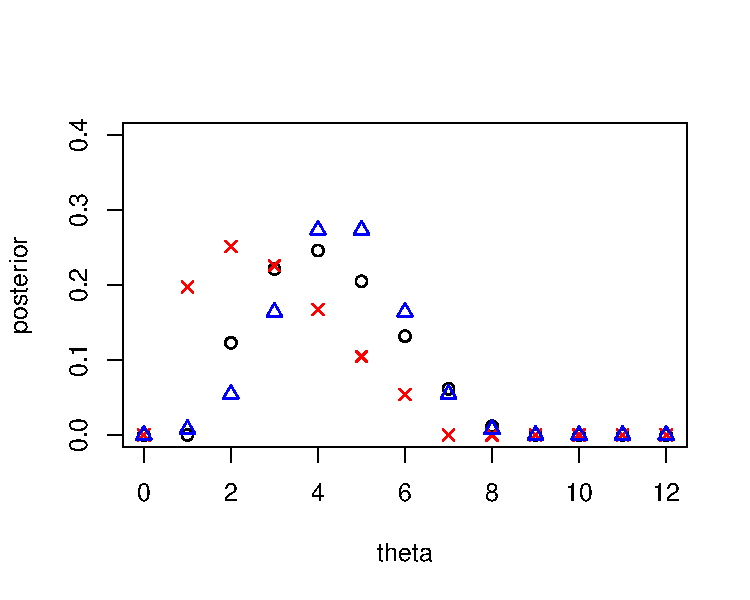
\includegraphics[width=.5\linewidth]{figure/plotsss-1} 

\end{knitrout}

\item This confirms what I speculated on in the previous problem. The one die prior matches up closest to the normalized likelihood function. This is because this prior is the least informative - it just puts a discrete uniform distribution values of $\theta$ between $1$ and $6$. This allows the likelihood to take the primary role in shaping the posterior distribution.

\begin{knitrout}\footnotesize
\definecolor{shadecolor}{rgb}{0.969, 0.969, 0.969}\color{fgcolor}
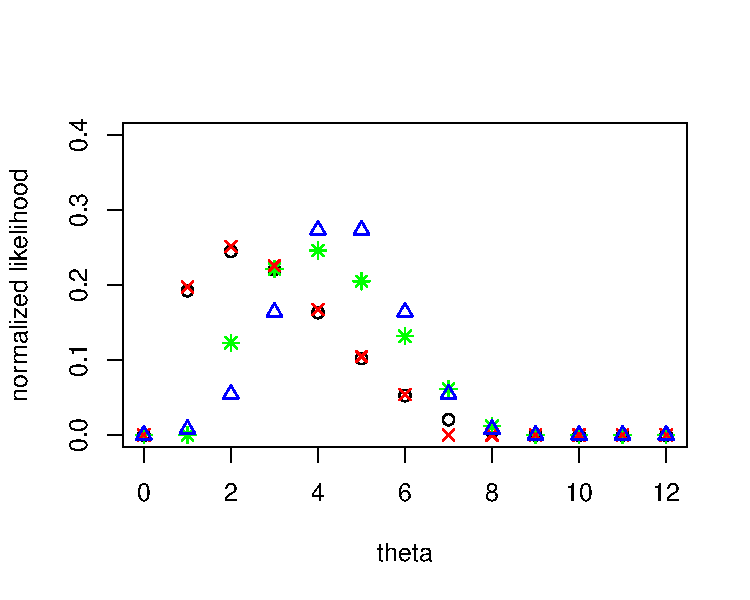
\includegraphics[width=.5\linewidth]{figure/plotnormpost-1} 

\end{knitrout}

\item See attached.


\end{enumerate}

\end{doublespacing}

\end{document}
